\documentclass[a4paper]{article}

\usepackage{ReportTemplate}

\usepackage{setspace}
\usepackage{amsmath}
\usepackage[hidelinks]{hyperref}

\title{Project 1:语音端点检测}
\name{姓名}
\studentid{学号}

\begin{document}

\maketitle

\section{LaTeX写作示例}

本章提供使用LaTeX书写报告时可能使用的各种文档对象的使用示例。\textbf{请在报告写作完成后删
除本章。}

\subsection{公式}

示例如式\ref{eq:公式引用名}。

\begin{equation}
  \pi = \dfrac{3.1415926}{1}
  \label{eq:公式引用名}
\end{equation}

\subsection{图像}

示例如图\ref{fig:图片引用名}。

\begin{figure}[htb]
  \centering
  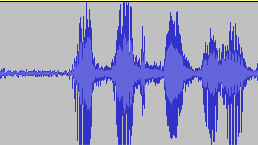
\includegraphics[scale=0.7]{figs/voice.png}
  \caption{图片标题}
  \label{fig:图片引用名}
\end{figure}

\subsection{表格}

示例如表\ref{tab:表引用名}。

\begin{table}[th]
  \caption{表标题}
  \label{tab:表引用名}
  \centering
  \begin{tabular}{ l c r }
    \toprule
    \textbf{左对齐} & \textbf{居中对齐} & \textbf{右对齐} \\
    \midrule
    内容 & 内容 & 内容 \\
    内容 & 内容 & 内容 \\
    \bottomrule
  \end{tabular}
\end{table}

\subsection{代码}

示例如下。

\begin{lstlisting}[language=python]
# 这是注释
def func(a, b):
    print("Hello, world!")
\end{lstlisting}

\section{基于线性分类器和语音短时能量的简单语音端点检测算法}

\subsection{数据预处理及特征提取}

本节介绍任务1中你对输入数据进行了哪些预处理步骤,提取了什么特征。对每种预处理步骤,请简要
介绍该步骤的效果或功能;对每种特征,请简要介绍该特征的定义和/或该特征对人耳听觉造成的直观
感受。\textbf{写作完成后,请删除本段。}

\subsection{算法描述}

请描述你的语音端点检测算法。若不止一种,可继续分节。请尽可能使用伪代码描述。如有必要,可以
贴出少量程序代码。\textbf{写作完成后,请删除本段。}

\subsection{实验结果}

请使用表格等形式给出你的算法在开发集上的性能表现。\textbf{写作完成后,请删除本段。}

\section{基于统计模型分类器和语音频域特征的语音端点检测算法}

\subsection{数据预处理及特征提取}

本节介绍任务2中你对输入数据进行了哪些预处理步骤,提取了什么特征。对每种预处理步骤,请简要
介绍该步骤的效果或功能;对每种特征,请简要介绍该特征的定义。\textbf{写作完成后,请删除本段
。}

\subsection{算法描述}

请描述你的语音端点检测算法。若不止一种,可继续分节。请尽可能使用伪代码描述。如有必要,可以
贴出少量程序代码。\textbf{写作完成后,请删除本段。}

\subsection{实验结果}

请使用表格等形式给出你的算法在开发集上的性能表现。\textbf{写作完成后,请删除本段。}

\end{document}
